  \begin{figure}
    \centering

    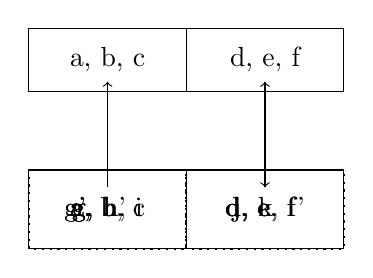
\begin{tikzpicture}
      \onslide<8-> {
        % Block 1
        \draw[] (0,0)  rectangle ++(2,0.8) node[pos=.5] (b1) {a, b, c};
      }

      \onslide<12-> {
        % Block 2
        \draw[] (2,0)  rectangle ++(2,0.8) node[pos=.5] (b2) {d, e, f};
      }

      % NOTE: Tikz does not like \only<>/\onslide<> within a node's text (even
      % if the output seems correct. So to not get compiler errors it must be
      % copy-pasted...

      % Memory 1
      \draw[dotted, thick] (0,-2) rectangle ++(2,1) node[pos=.5] (M1) {};

      \onslide<2> {
        \draw[] (0,-2) rectangle ++(2,1) node[pos=.5] (M1) {a\phantom{, b, c}};
      }
      \onslide<3> {
        \draw[] (0,-2) rectangle ++(2,1) node[pos=.5] (M1) {a, b\phantom{, c}};
      }
      \onslide<4-7> {
        \draw[] (0,-2) rectangle ++(2,1) node[pos=.5] (M1) {a, b, c};
      }

      \onslide<9,18> {
        \draw[] (0,-2) rectangle ++(2,1) node[pos=.5] (M1) {g\phantom{, h, i}};
      }
      \onslide<10,17> {
        \draw[] (0,-2) rectangle ++(2,1) node[pos=.5] (M1) {g, h\phantom{, i}};
      }
      \onslide<11-16> {
        \draw[] (0,-2) rectangle ++(2,1) node[pos=.5] (M1) {g, h, i};
      }

      \onslide<23> {
        \draw[] (0,-2) rectangle ++(2,1) node[pos=.5] (M1) {g'\phantom{, h', i}};
      }
      \onslide<24-> {
        \draw[] (0,-2) rectangle ++(2,1) node[pos=.5] (M1) {g', h'\phantom{, i}};
      }

      % Memory 2
      \draw[dotted, thick] (2,-2) rectangle ++(2,1) node[pos=.5] (M2) {};

      \onslide<5> {
        \draw[] (2,-2) rectangle ++(2,1) node[pos=.5] (M2) {d\phantom{, e, f'}};%
      }
      \onslide<6,21> {
        \draw[] (2,-2) rectangle ++(2,1) node[pos=.5] (M2) {d, e\phantom{, f'}};%
      }
      \onslide<7-11,20> {
        \draw[] (2,-2) rectangle ++(2,1) node[pos=.5] (M2) {d, e, f\phantom{'}};%
      }
      \onslide<22-> {
        \draw[] (2,-2) rectangle ++(2,1) node[pos=.5] (M2) {d, e, f'};%
      }

      \onslide<13, 15> {
        \draw[] (2,-2) rectangle ++(2,1) node[pos=.5] (M2) {j\phantom{, k, l}};
      }
      \onslide<14> {
        \draw[] (2,-2) rectangle ++(2,1) node[pos=.5] (M2) {j, k\phantom{, l}};
      }

      % Arrows
      \onslide<8>  { \draw[->] (M1) edge (b1); }
      \onslide<12> { \draw[->] (M2) edge (b2); }
      \onslide<20> { \draw[->] (b2) edge (M2); }
    \end{tikzpicture}
  \end{figure}
